% !TEX root = main.tex
\documentclass{article}
\usepackage{../include/report_style}

\newcommand{\TODO}[1]{\textcolor{red}{TODO: #1}} % for comments

\title{Lean Applications in the Department of Defense}
\author{Juan Carlos Cruz - ira406}
\date{ME 5703 Lean Product Development and Service Systems}

\begin{document}
	\maketitle
	\noindent%

	\begin{abstract}
		This report investigates the implementation of lean and six sigma principles within the Department of Defense (DoD) and its affiliated organizations through a scientometric analysis of the literature and then case study analysis of notable works from that search.
		Using a structured search methodology across 465 documents from the ProQuest database spanning 1992-2025, the study identifies publication trends, document types, and thematic patterns in lean six sigma literature within defense contexts. 
		The analysis reveals three predominant themes: Management and Leadership (54\%), Process Improvement (35.9\%), and Continuous Learning (9.2\%).
		Case studies from each theme include significant efficiency improvements in depot operations, enhanced contractor relationship management reflecting keiretsu principles, and lean approaches to knowledge management and data accessibility. 
		Despite the inherent challenges of implementing lean methodologies in bureaucratic defense organizations, this research provides evidence that lean and six sigma principles have been effectively introduced to various aspects of DoD operations, contributing to efficiency, waste reduction, and more effective process management. 
		These findings suggest that while contextual adaptation is necessary, lean thinking offers valuable frameworks for addressing the DoD's complex operational challenges and resource constraints.
	\end{abstract}

	% Introduction
	\section{Introduction}

		The Department of Defense (DoD), which includes the U.S. Army, Navy, Air Force, Marine Corps, Space Force, National Security Agency, Defense Intelligence Agency, National Geospatial-Intelligence Agency, and National Reconnaissance Office, is traditionally viewed as a bureaucratic and slow-moving organization due to its sheer size and complexity.

		In this report we aim to investigate the implementation of lean and six-sigma principles within the DoD and its affiliated organizations to identify if these principles have been successful in improving the efficiency and effectiveness of the DoD.
		To better understand research trends regarding lean and six-sigma implementation regarding the DoD, a scientometric review is conducted following the procedure outlined in \cite{MA2023104828}.
		The review begins by selecting an appropriate database, tailoring a search term criteria, filtering the results, and then analyzing the key research themes appearing across the resulting works.
		After the review we select notable works to examine as case studies in lean methodologies. 

		The complete citation dataset, analysis code, and figures can be found at \url{https://github.com/jc-cr/lean_dod_paper}.

	\section{Scientometric Analysis}

	\subsection{Setup}

		ProQuest was selected as the primary database for this search as it yielded the most results, 481 total, including Theses, Trade journals, Scholarly Articles, and Conference Papers.

		The author also reviewed the Web of Science, Lens, and the Defense Technical Information Center, but found these to have insufficient paper results for this analysis.

		One downside to this search method is that valuable "Grey literature" including government web articles and reports are not included within the analysis, this limitation will be covered in the final report by including such literature in the final review.

		The search term used in ProQuest was as follows:

		\begin{minipage}{\linewidth}
		\begin{spacing}{0.8}
		\noindent\texttt{AB("Department of Defense" OR "DoD" OR "DOD" OR "U.S. Army" OR} \\
		\texttt{"Department of the Army" OR "U.S. Navy" OR "Department of the Navy" OR} \\
		\texttt{"U.S. Air Force" OR "Department of the Air Force" OR "U.S. Marine Corps" OR} \\
		\texttt{"U.S. Space Force" OR "National Security Agency" OR "NSA" OR} \\
		\texttt{"Defense Intelligence Agency" OR "DIA" OR "National Geospatial-Intelligence} \\
		\texttt{Agency" OR "NGA" OR "National Reconnaissance Office" OR "NRO")} \\
		\texttt{AND FT("six sigma" OR "6$\sigma$" OR "lean six sigma" OR} \\
		\texttt{"continuous process improvement" OR "LSS") AND LA(EN)}
		\end{spacing}
		\end{minipage}

		The resulting papers were inspected and cleaned manually for irrelevant documents or duplicates, leaving 465 documents to analyze.
		The results were exported to a xlsx file and then analyzed with a python script.

		The python analysis program was setup to output graphs related to the following items:

		\begin{itemize}
			\item \textbf{Publication Trend Analysis}: Temporal distribution of publications by year, including trend lines and 3-year moving averages to identify patterns in research activity.
			
			\item \textbf{Document Type Classification}: Analysis of publication types (e.g., journal articles, case studies, dissertations).
			
			\item \textbf{Keyword Analysis}: Extraction and frequency analysis of keywords from abstracts, including removal of common stopwords and use of lemmatization for term normalization.
			
			\item \textbf{Network Analysis}: Construction of keyword co-occurrence networks to visualize relationships between concepts in the literature, with filtering to highlight the most significant connections.
			
			\item \textbf{Topic Modeling}: Latent Dirichlet Allocation (LDA) modeling to identify underlying thematic structures across the corpus of abstracts.
			
			\item \textbf{Thematic Trend Analysis}: From prior analysis, analysis of the identified themes in the literature over time.

			\item \textbf{Thematic Distribution}: Distribution of themes across the corpus of abstracts.
		\end{itemize}

		The results and figures generated from these analysis methods are presented in the following sections.

	\subsection{Analysis}

		As seen in \figref{fig:publication_trend}, from the earliest publications found in 1992 up to 2025, there has been an increasing trend for lean six sigma related publication related to the DoD and it's affiliated organizations.
		The year 2017 saw the most amount of publication related to lean six sigma and the DoD.
		Interestingly, since 2017 there has been a downward trend in lean six sigma literature.

		\begin{figure}[htbp]
			\centering
			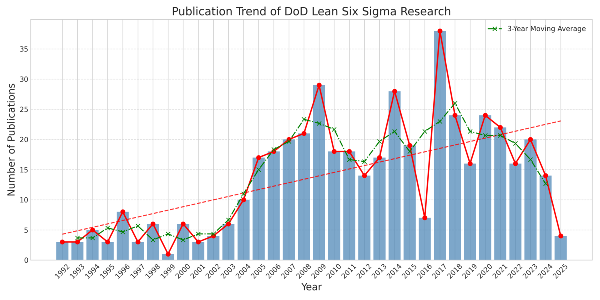
\includegraphics[width=0.9\linewidth,height=0.9\textheight,keepaspectratio]{publication_trend}
			\caption{Publications in lean six sigma from database search}
			\label{fig:publication_trend}
		\end{figure}

		The majority of the publication types found in the ProQuest database are Dissertation/Thesis, with Feature, and General Information documents following after.
		This is visualized in \figref{fig:document_type}
		The trends over time for the different document classes is shown in \figref{fig:document_type_trend}.

		\begin{figure}[htbp]
			\centering
			\begin{subfigure}[b]{0.48\textwidth}
				\centering
				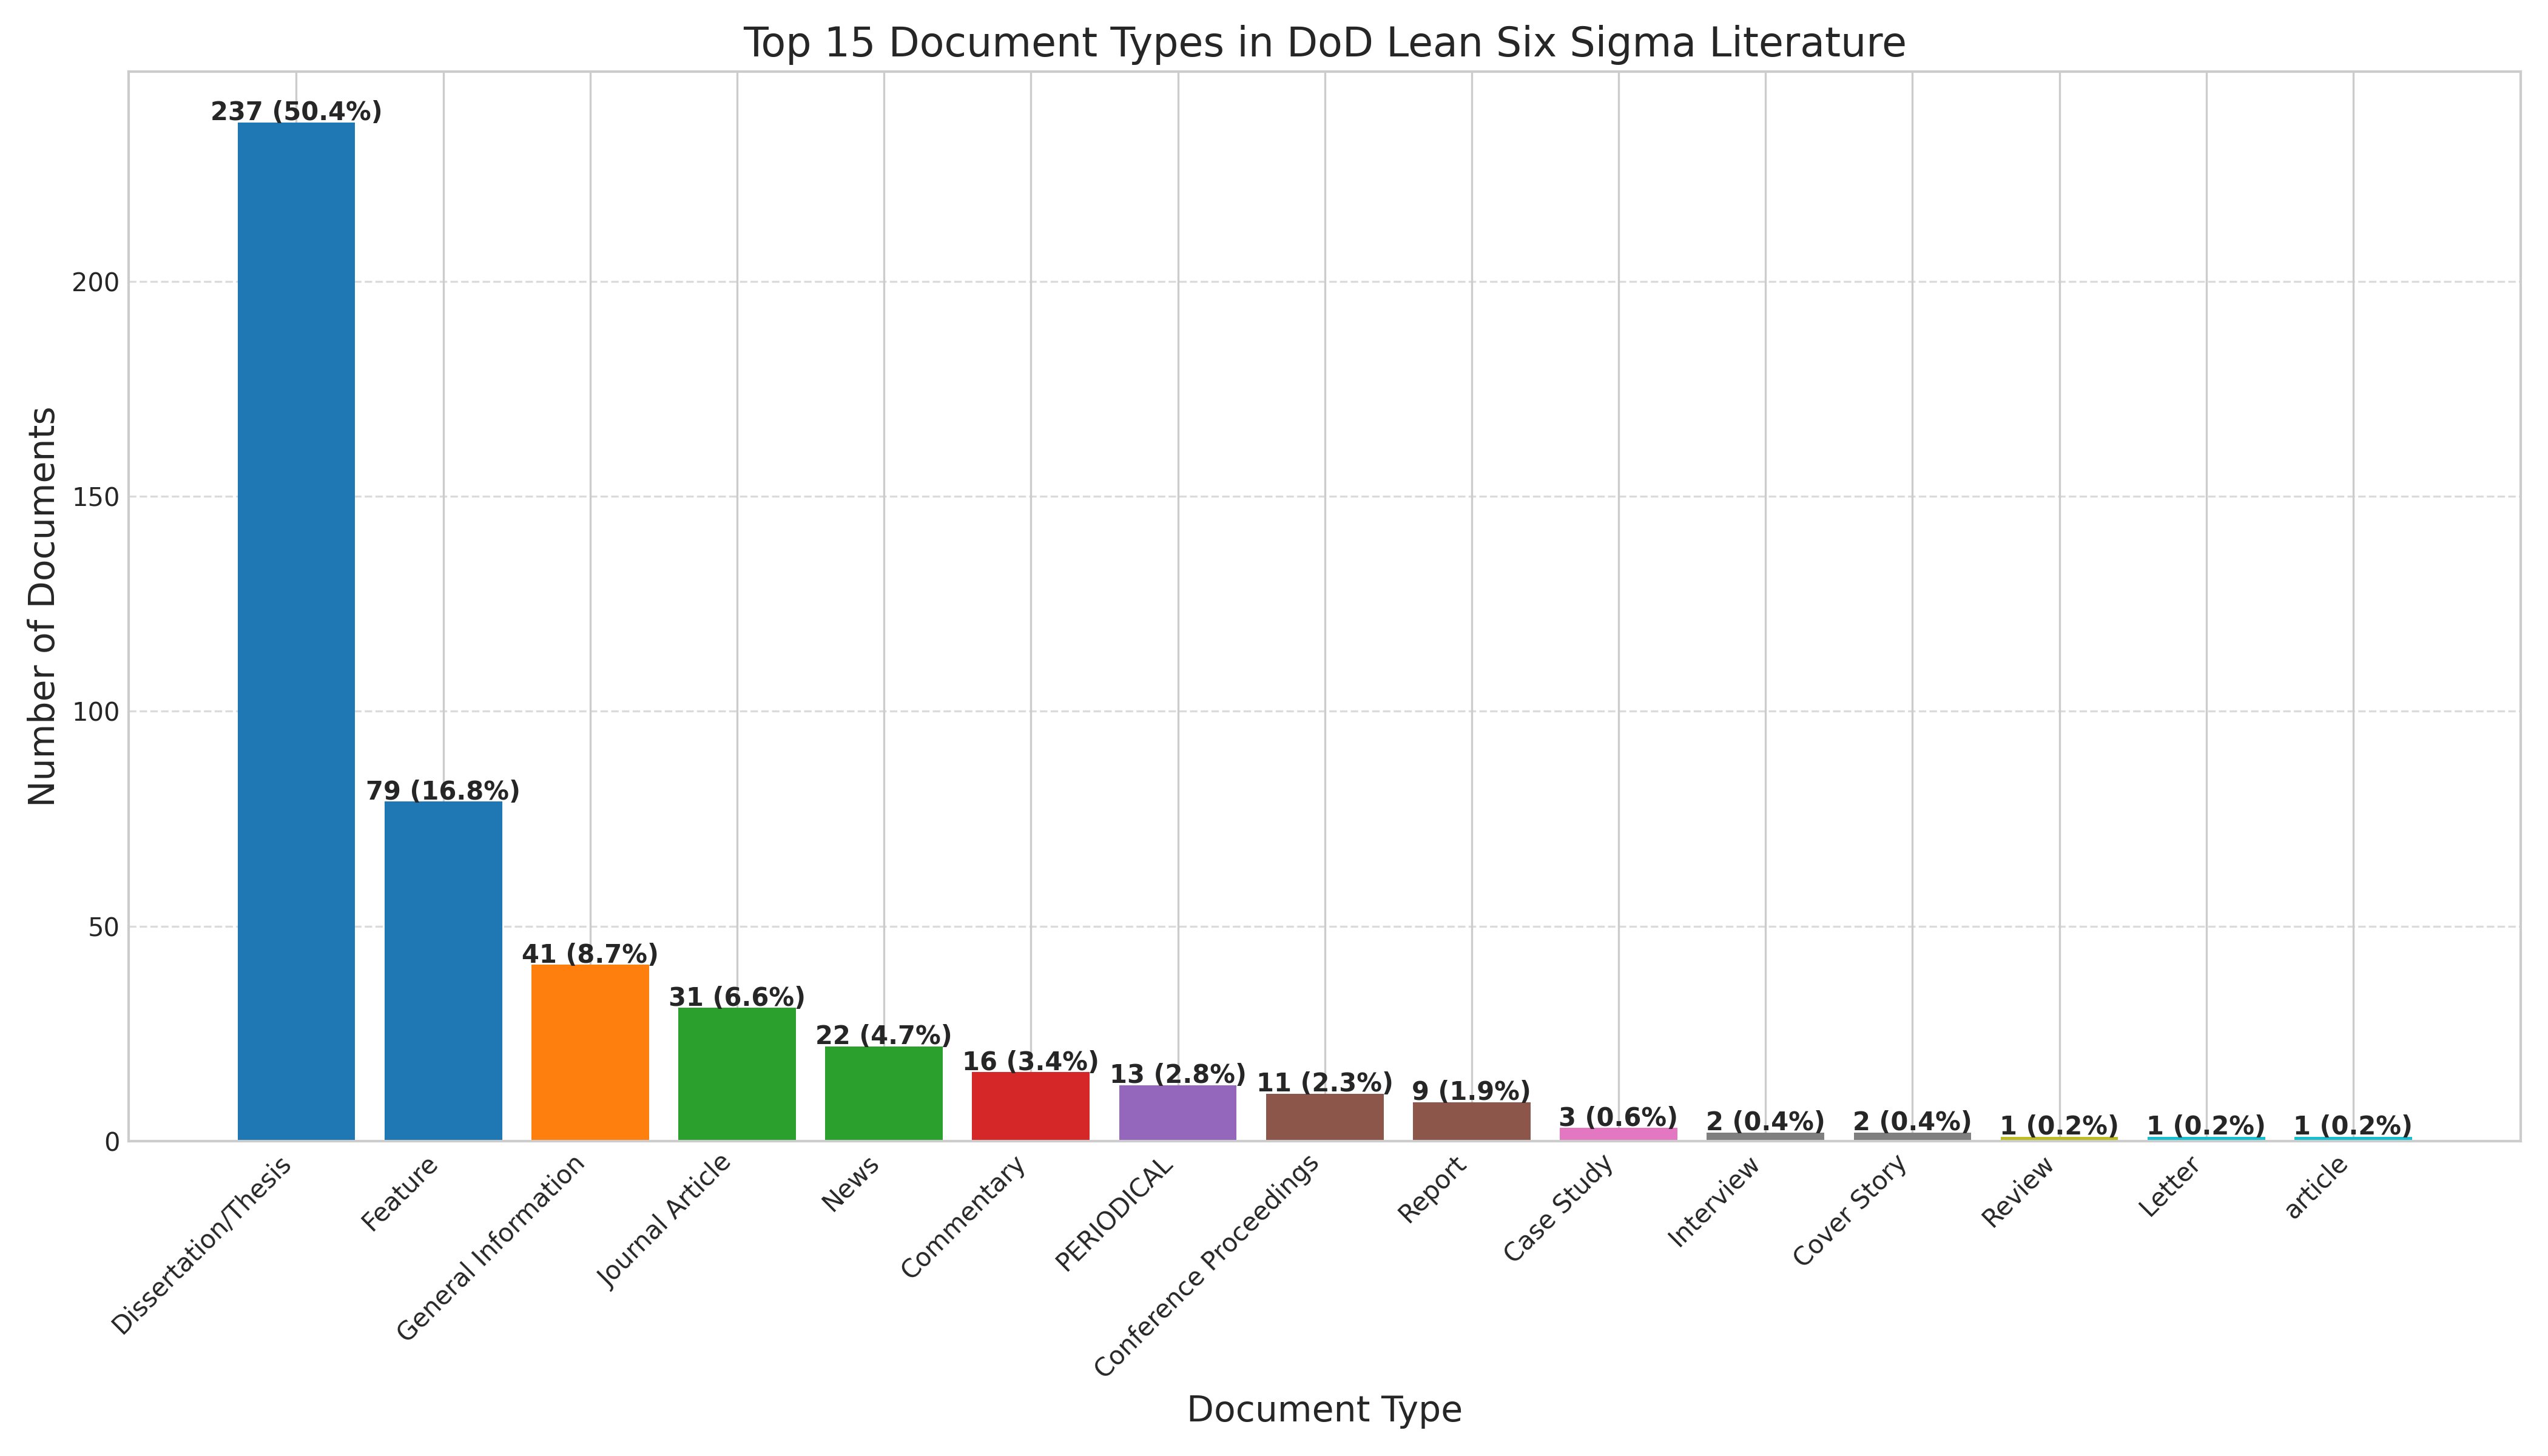
\includegraphics[width=\textwidth,height=0.35\textheight,keepaspectratio]{document_type_distribution_bar}
				\caption{Types of publications found in the database search}
				\label{fig:document_type}
			\end{subfigure}
			\hfill
			\begin{subfigure}[b]{0.48\textwidth}
				\centering
				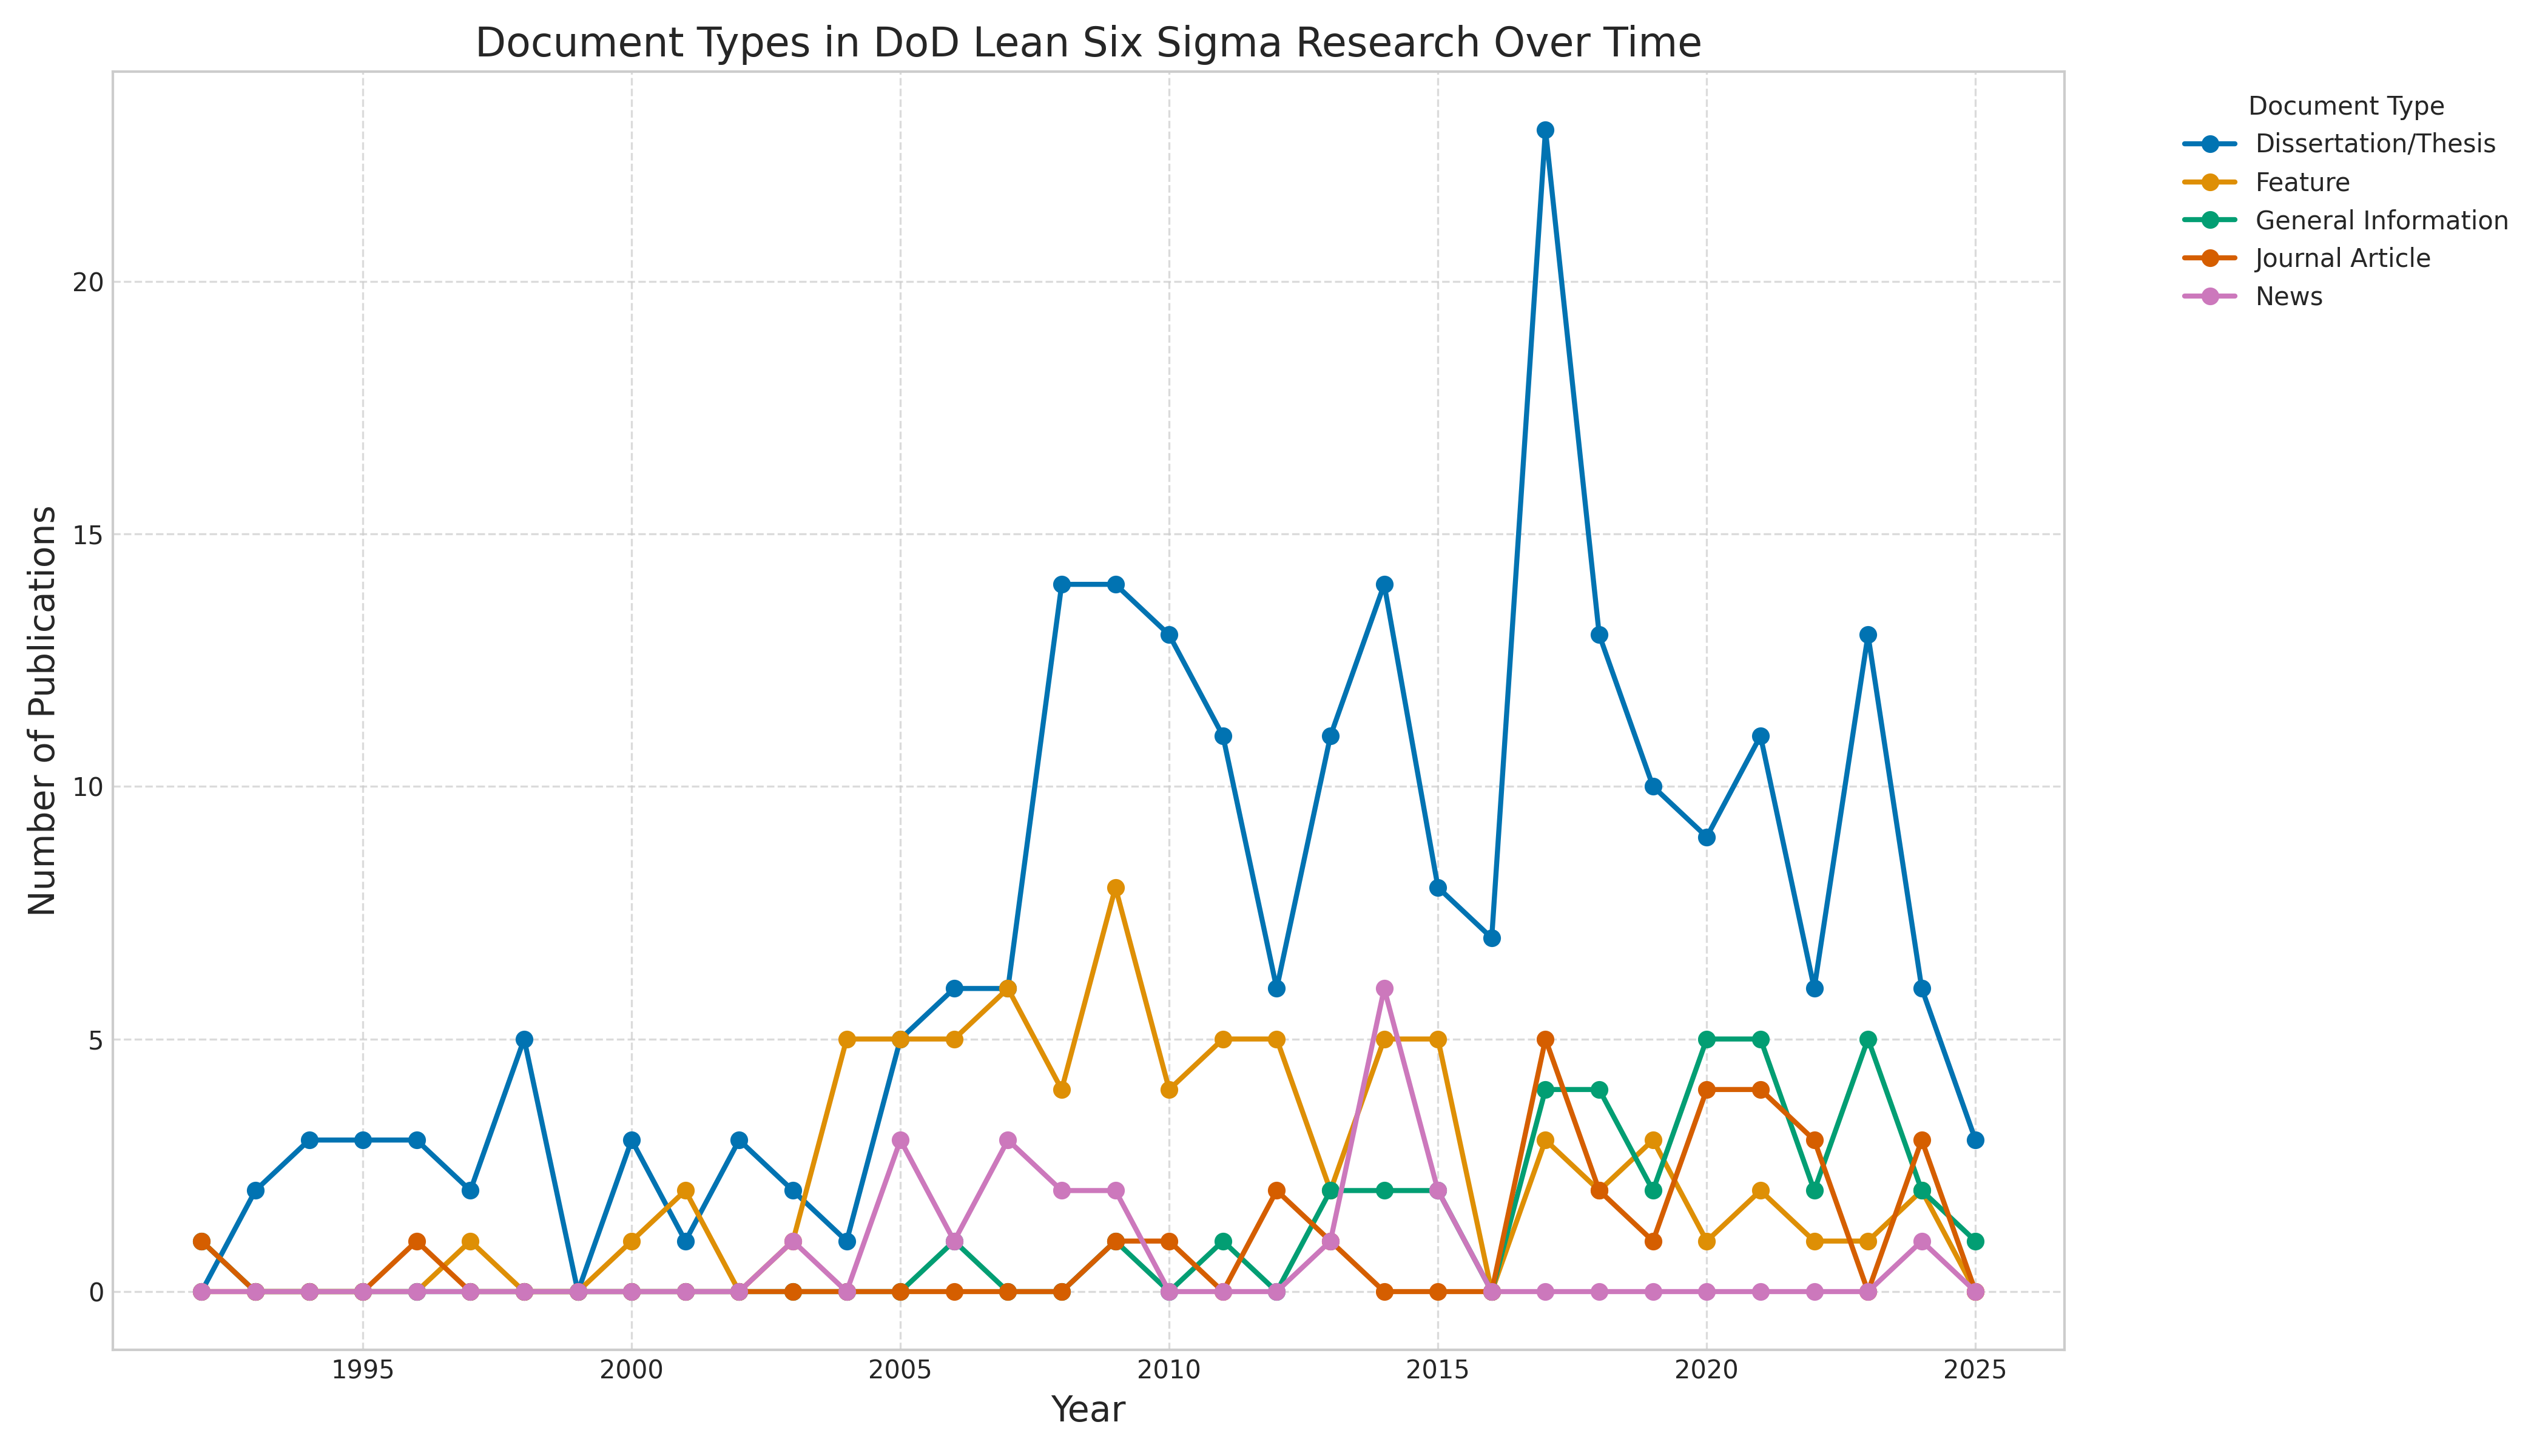
\includegraphics[width=\textwidth,height=0.35\textheight,keepaspectratio]{document_type_trends}
				\caption{Trend over time for the different document types}
				\label{fig:document_type_trend}
			\end{subfigure}
			\caption{Analysis of document types and their trends over time}
			\label{fig:document_analysis}
		\end{figure}


		Analyzing the keywords present in the document abstracts, \figref{fig:keyword_freq} shows that \textit{system}, \textit{process}, and \textit{management} appear with the highest frequency across all documents.
		From the co-occurrence network in \figref{fig:keyword_network}, we observe that \textit{management}, \textit{data}, and \textit{process} have a high betweenness centrality, indicating they serve as important bridges connecting other keywords in the literature. This suggests these concepts play central roles in linking different aspects of lean six sigma implementation within DoD contexts.
		A Latent Dirichlet Allocation method uncovered the following key topic areas, shown in \figref{fig:topics}, \textit{Organization, System, Process/Management,} and \textit{Operation}.

		\begin{figure}[htbp]
			\centering
			\begin{subfigure}[b]{0.32\textwidth}
				\centering
				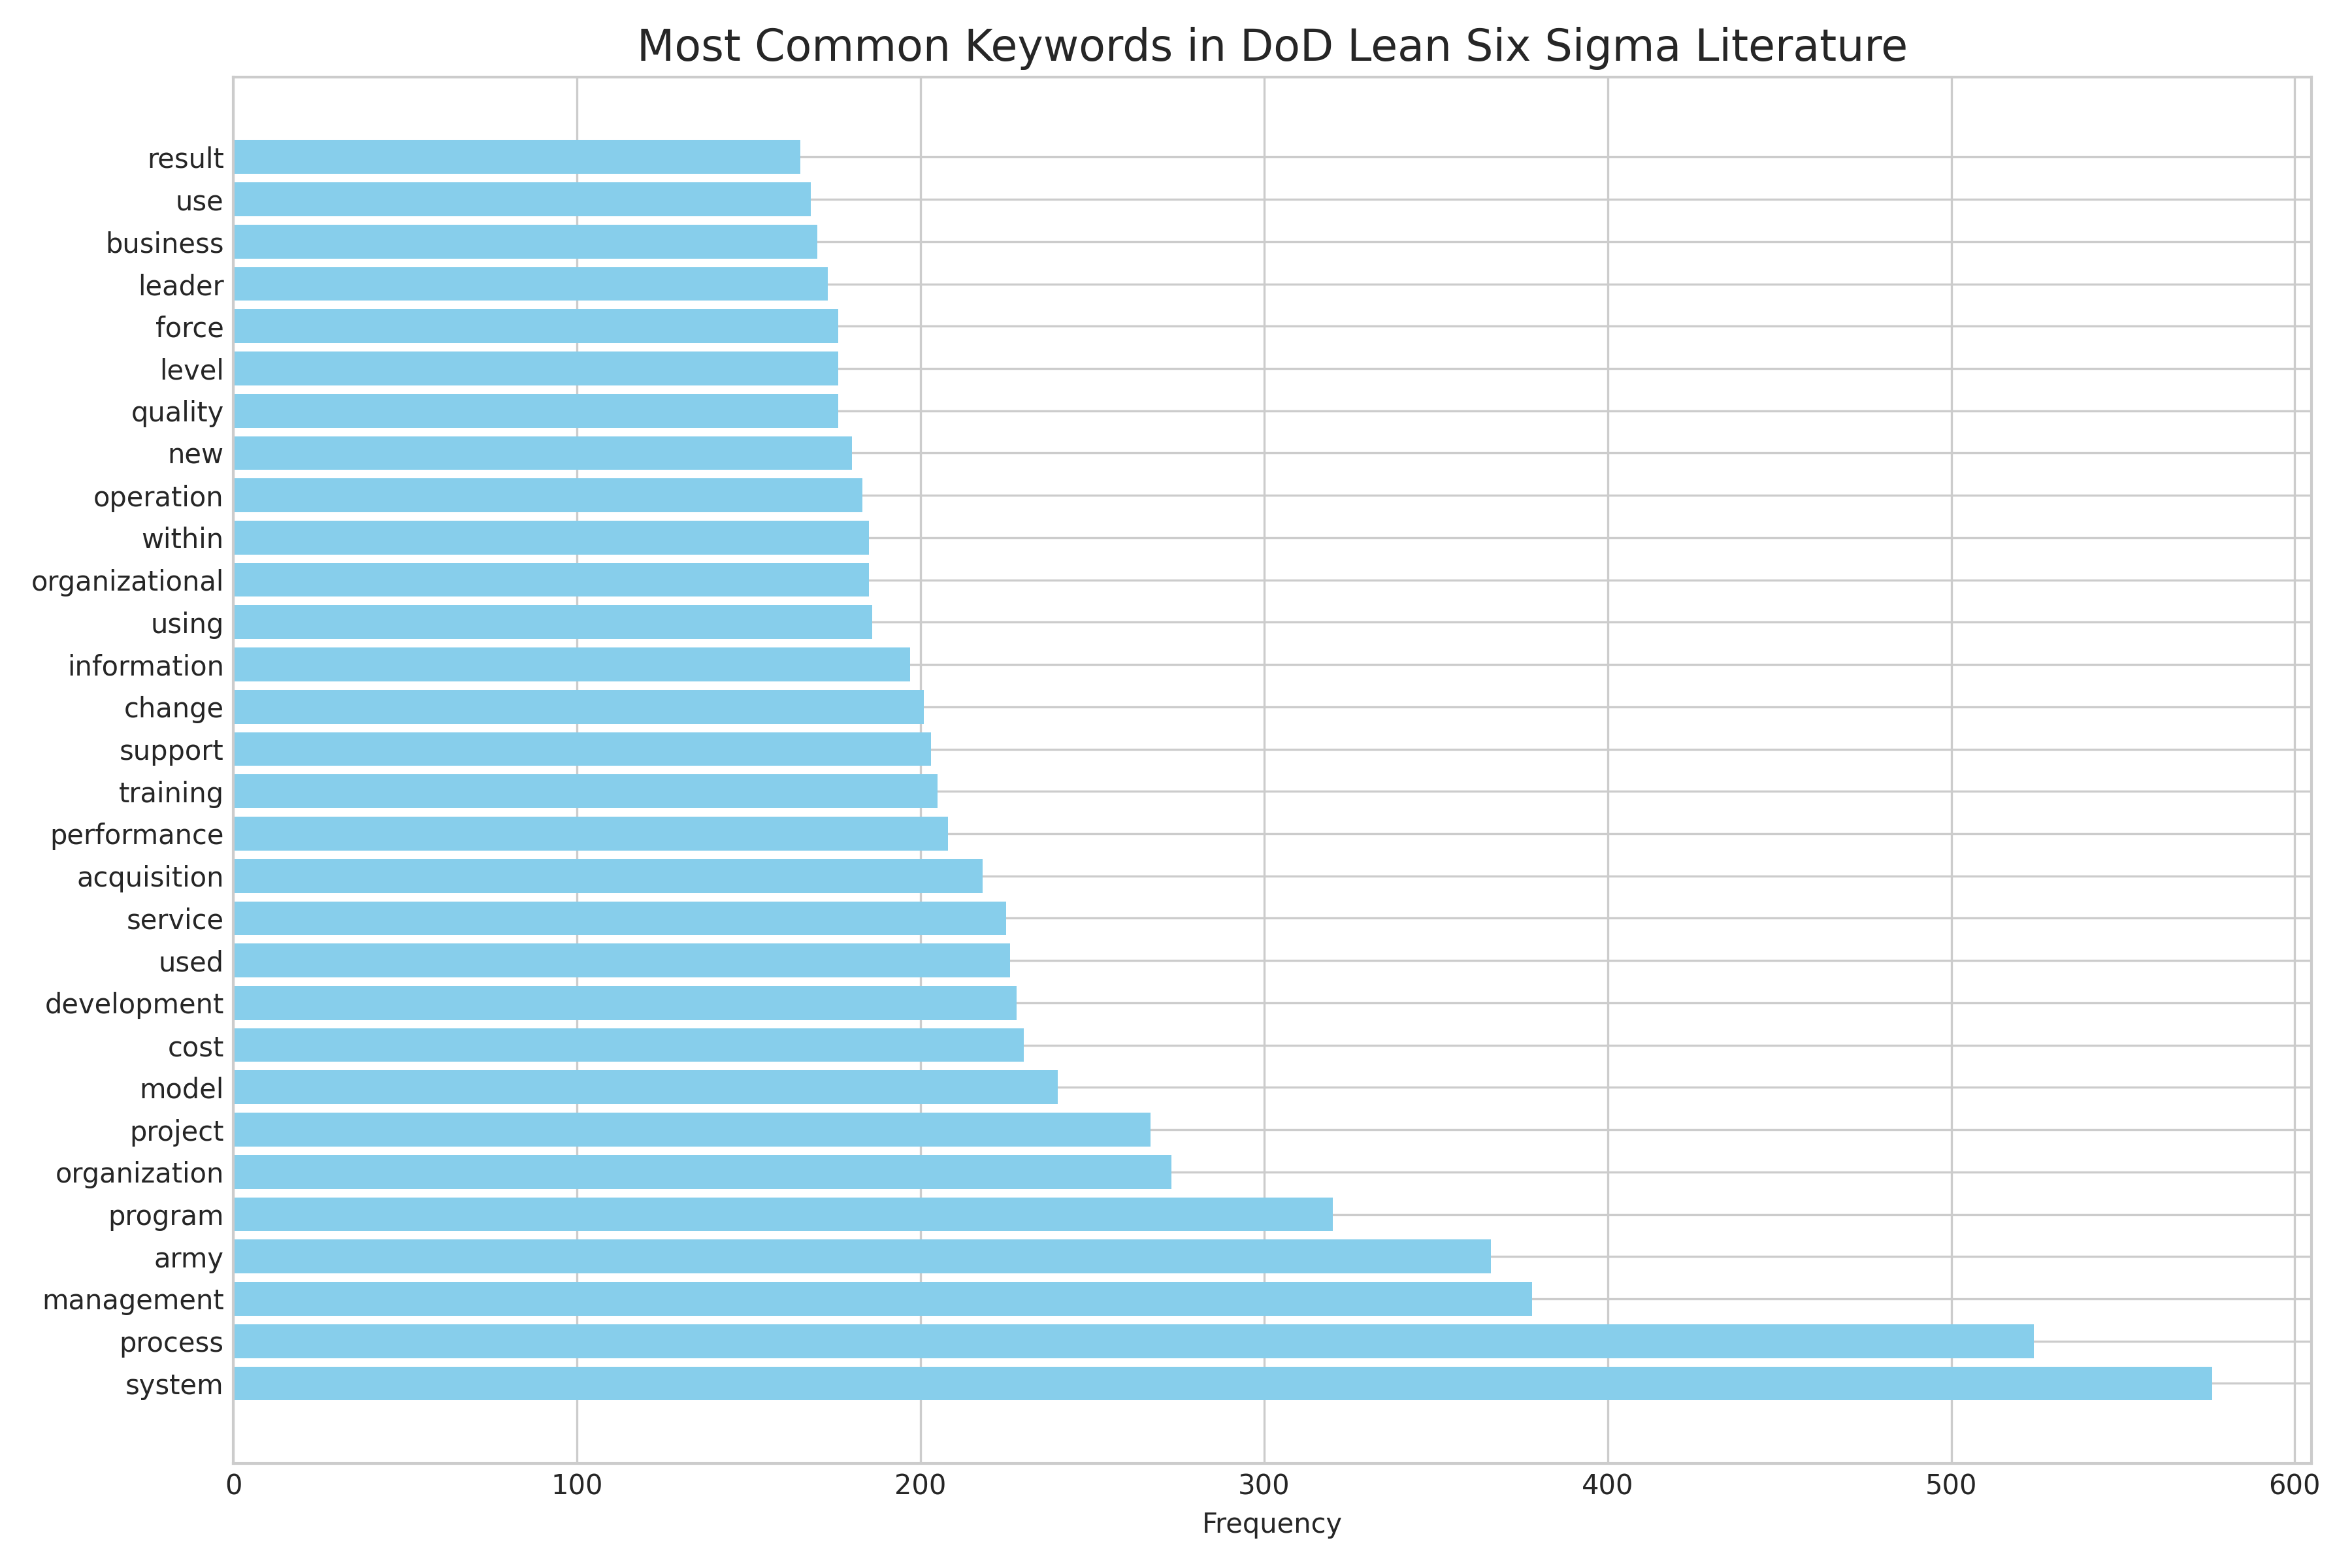
\includegraphics[width=\textwidth,height=0.25\textheight,keepaspectratio]{keyword_frequency}
				\caption{Keyword appearance frequency}
				\label{fig:keyword_freq}
			\end{subfigure}
			\hfill
			\begin{subfigure}[b]{0.32\textwidth}
				\centering
				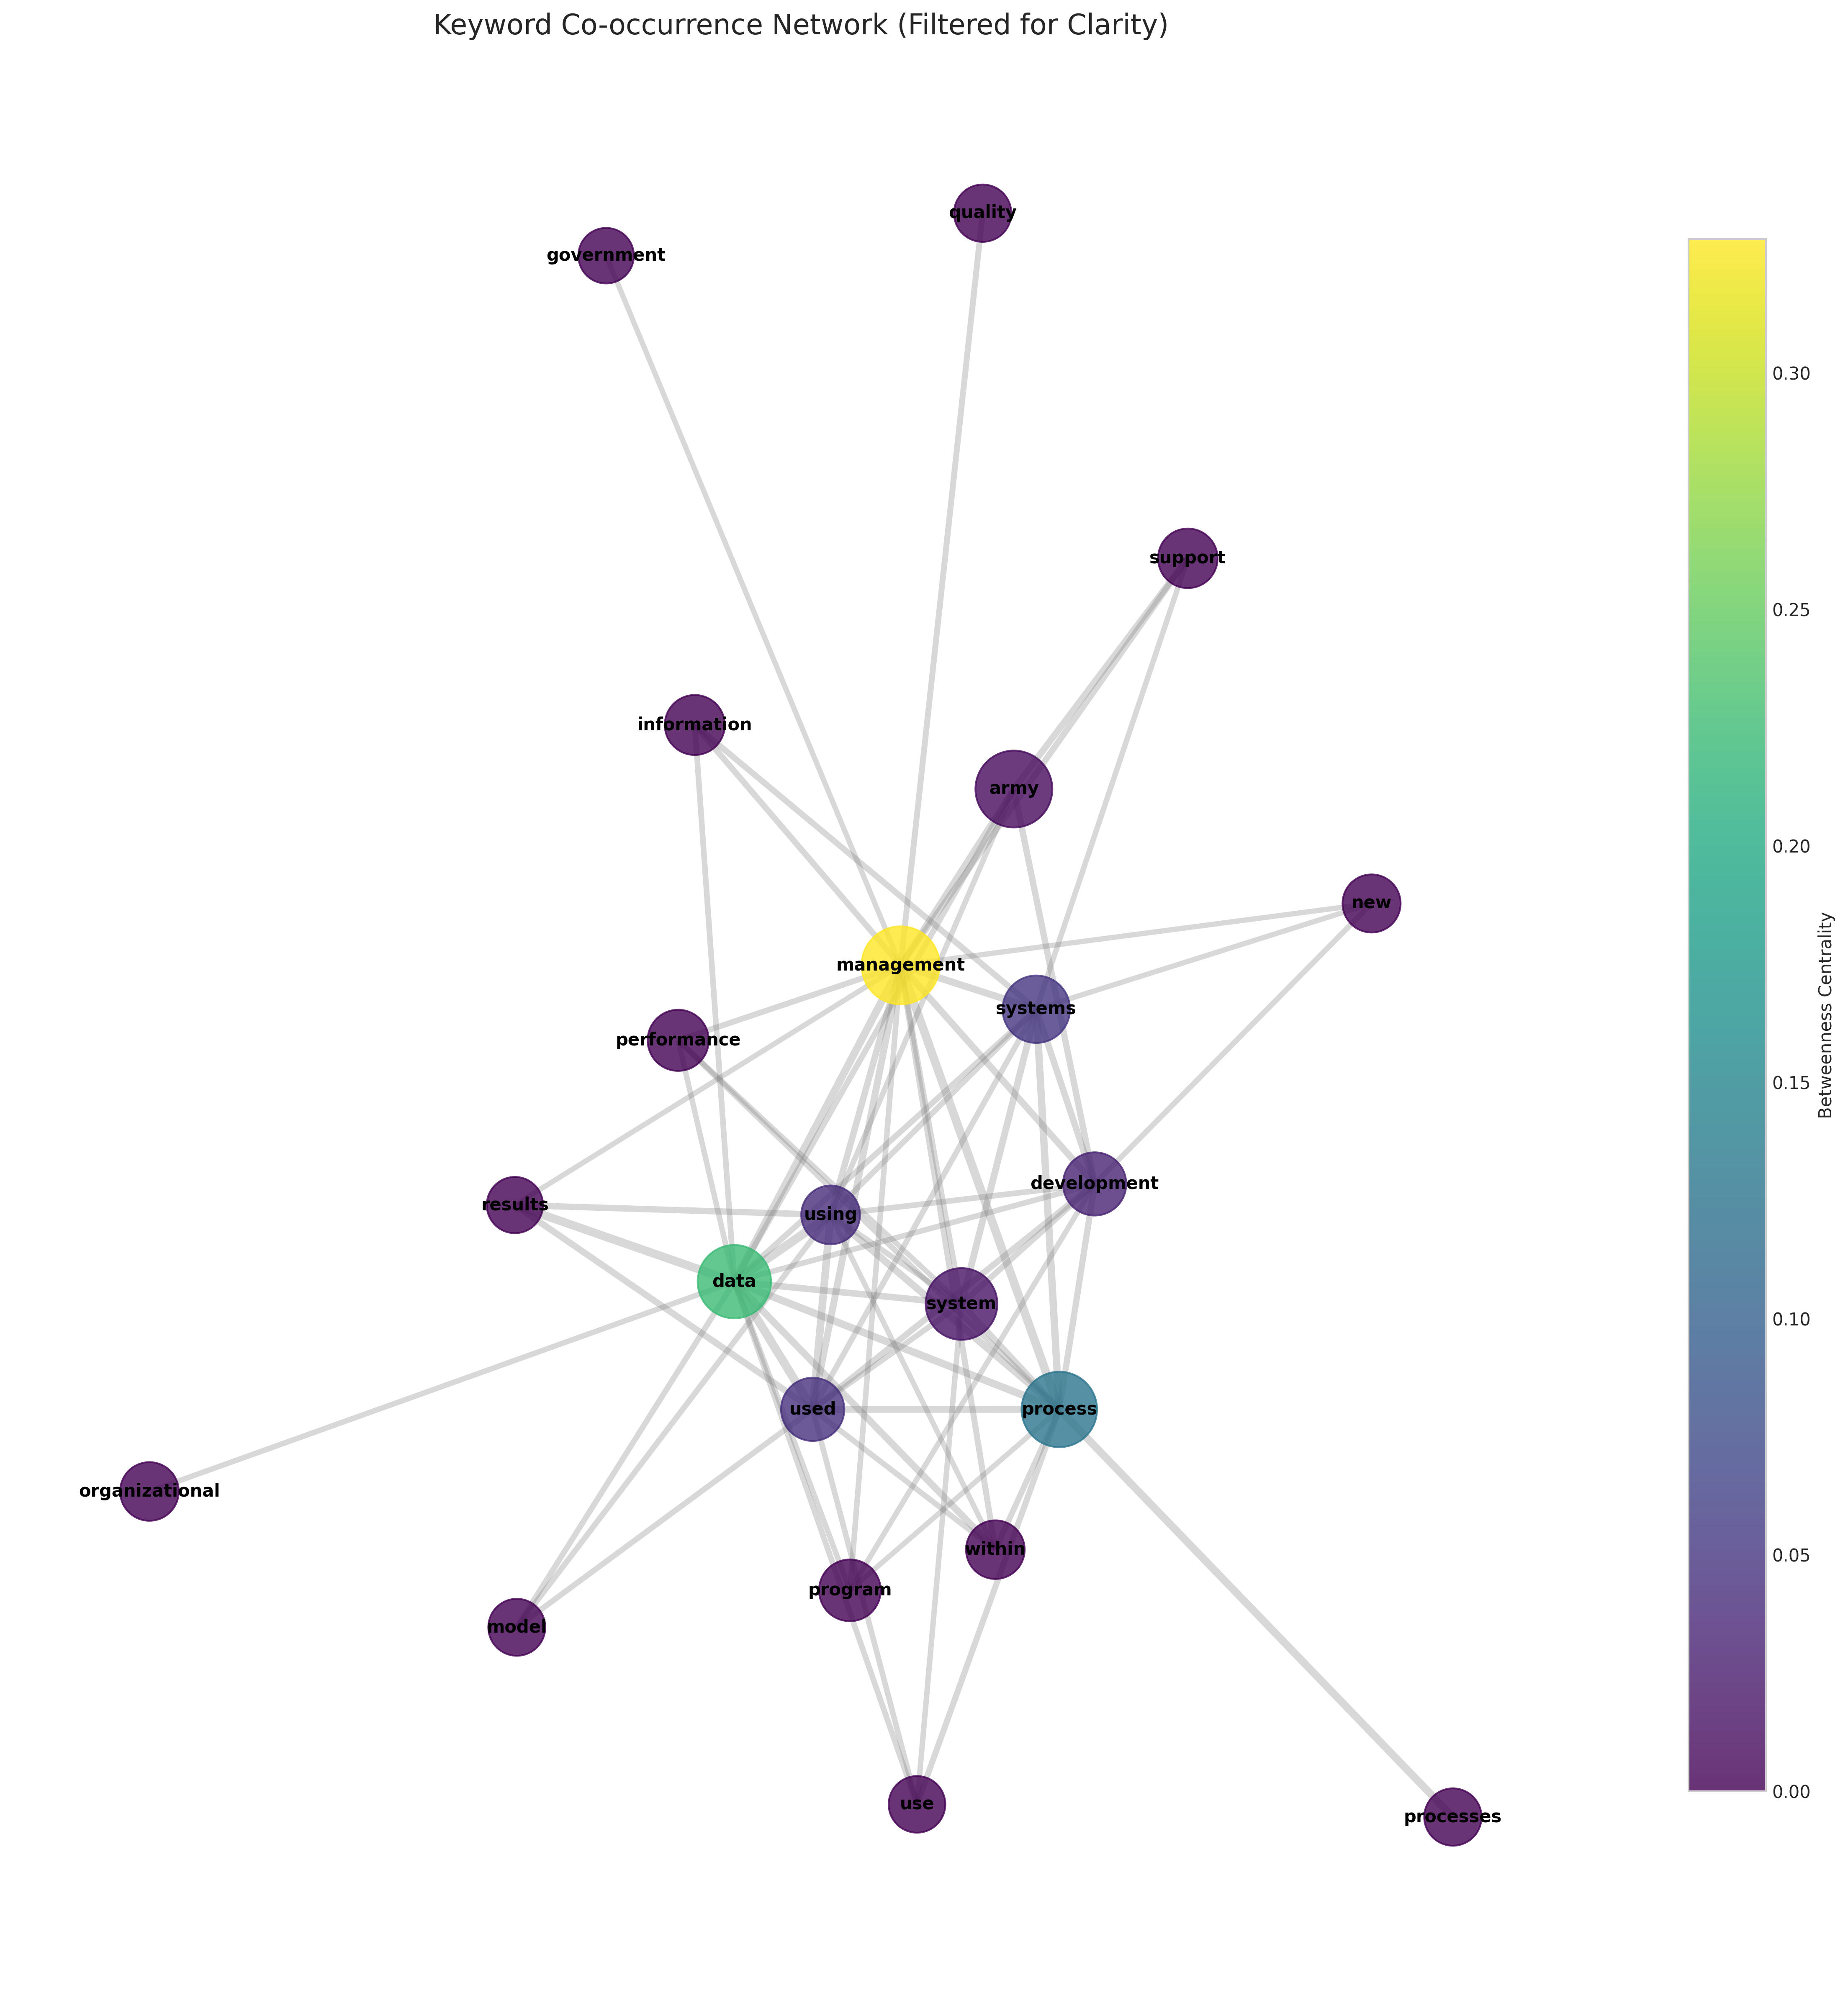
\includegraphics[width=\textwidth,height=0.25\textheight,keepaspectratio]{keyword_network}
				\caption{Keyword co-occurrence network}
				\label{fig:keyword_network}
			\end{subfigure}
			\hfill
			\begin{subfigure}[b]{0.32\textwidth}
				\centering
				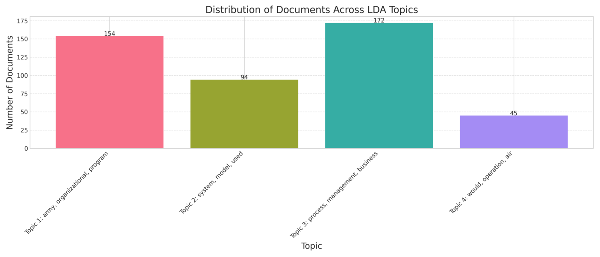
\includegraphics[width=\textwidth,height=0.25\textheight,keepaspectratio]{topic_distribution}
				\caption{Topic distribution from LDA analysis}
				\label{fig:topics}
			\end{subfigure}
			\caption{Keyword analysis and topic modeling results}
			\label{fig:keyword_analysis}
		\end{figure}

		Using all the prior analysis points, we determined three main themes in the lean six sigma literature: \textit{Management and Leadership, Process Improvement,} and \textit{Continuous Learning}. 
		Using these three themes, a keyword-based categorization algorithm was applied to classify each document according to the most similar theme.

		As visualized in \figref{fig:theme_distribution_bar}, the majority of the papers (54\%) corresponded to the \textit{Management and Leadership} theme, 35.9\% fell into the \textit{Process Improvement} theme, and 9.2\% fell into the \textit{Continuous Learning} theme.
		The distribution of themes over the years is shown in \figref{fig:theme_trends}.
		The following sections will take notable papers from each theme and analyze them for their impact and lean principles used.

		\begin{figure}[htbp]
			\centering
			\begin{subfigure}[b]{0.48\textwidth}
				\centering
				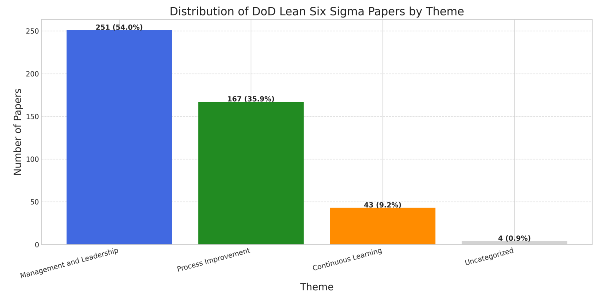
\includegraphics[width=\textwidth,height=0.35\textheight,keepaspectratio]{theme_distribution_bar.pdf}
				\caption{Distribution of themes in the literature}
				\label{fig:theme_distribution_bar}
			\end{subfigure}
			\hfill
			\begin{subfigure}[b]{0.48\textwidth}
				\centering
				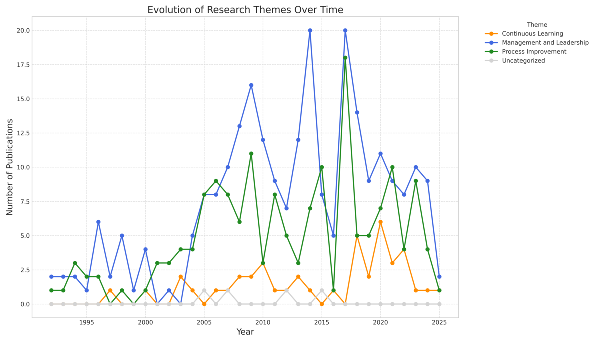
\includegraphics[width=\textwidth,height=0.35\textheight,keepaspectratio]{theme_trends_over_time.pdf}
				\caption{Theme trends over time}
				\label{fig:theme_trends}
			\end{subfigure}
			\caption{Thematic analysis of lean six sigma literature in DoD contexts}
			\label{fig:theme_analysis}
		\end{figure}

	\section{Management and Leadership}

		Toyota's approach to management can be described as Hourensou style management that is multidimensional in nature.
		Managers communicate openly and information travels up, down, and sideways allowing for the necessary flow of information to the correct parties. 

		This is in contrast to traditional North American style of command and control style management where managers delegate out work and information with little input from subordinates.
		In fact, command-and-control style management also makes it difficult to achieve the necessary communication flows to suppliers and external partners.

		Since the DoD follows is composed of various military entities which traditionally operate on this command-and-control style organization, it can be difficult for lean methodologies to take root in such an entrenched system.
		In the following case studies gathered from our literature review, we see examples which offer insight and examples from lean thinking to existing systems in the DoD.


		\subsection{Leadership Development Strategies for Sustaining Organization Performance Through the Upper Echelon Theory \cite{McCants2024}}	

			In \cite{McCants2024}, the author conducted a survey into strategies that senior leaders use to transition new subordinate leaders into organizations, specifically focusing on the Department of the Army in the Military District of Washington. 
			This environment frequently experiences turnovers, creating potential disruptions to organizational continuity and performance.
			Through semi-structured interviews with eight military and civilian leaders, each with over eight years of experience in developing midlevel managers, the author identified five key themes essential for successful leadership transitions:

			\begin{itemize}
				\item Knowledge of organization during change
				\item Effective communication skills
				\item Flexible and adaptive leadership
				\item Having performance measures
				\item Formal and informal leader development
			\end{itemize}

			Although the study uses the idea of Upper Echelon Theory which describes orginization outcomes are influenced by top-level management characteristics \cite{uppere}, various themes from lean/six sigma align with the study.
			The emphasis on organizational knowledge mirrors Toyota's concept of \textit{genchi genbutsu} (go and see), where managers are expected to thoroughly understand operations before making decisions. 
			The focus on communication parallels Toyota's \textit{hourensou} approach to management, which facilitates multi-directional information flow (up, down, and lateral) that contrasts with traditional command-and-control structures.

			The study demonstrates that even in hierarchical structures like the Department of the Army, lean-inspired leadership development strategies can be successfully implemented to maintain operational continuity during leadership transitions.


		\subsection{Project Engineers on the Frontline: The Impact of Work-Related Stressors and Turnover Intentions: A Correlational Study \cite{Turner2024}}

			In \cite{Turner2024}, the author conducts a quantitative correlational study examining the relationship between work-related stressors and turnover intentions among project engineers who have worked in the DoD or for companies contracted by the DoD. 
			Project engineers in this work were engineers directly managing planning, budgets, execution and delivery of DoD projects.
			The study surveyed 69 project engineers to reveal a strong positive correlation between work stress and turnover intention.

			By going to the source and collecting data directly from project engineers, the author was able to identify one of the root causes of a serious problem affecting DoD projects—employee turnover due to work-related stress. 
			The study finds that the following factors have the most contribution to project engineer turnover intentions:

			\begin{itemize}
				\item Excessive workloads
				\item Tight deadlines
				\item Technical complexity
				\item Interpersonal conflict
				\item Insufficient resources
			\end{itemize}

			These findings align strongly with lean thinking principles, particularly Toyota's concept of \textit{muri} (overburden). 
			In the Toyota Production System, \textit{muri} is considered one of the three major wastes (along with \textit{muda} and \textit{mura}) that organizations must eliminate.
			Toyota managers understand that sustainable performance comes from creating a leveled workflow (\textit{heijunka}) that avoids the deadly waste of overburden on employees. 
			Overburdening employees beyond their capacity leads to stress, burnout, and ultimately higher turnover—exactly what Turner's study demonstrates empirically. 
			By identifying work-related stress as a key predictor of turnover intentions, this study provides evidence for a causal relationship that lean organizations can address through improved work design and management practices.


		\subsection{Understanding the Contracting Environment in the AFSB: Army Logistician \cite{Carlstedt2020}}

			The article of \cite{Carlstedt2020} provides insight into how the Army, a DoD organization, manages relations and contracts with it's suppliers.
			The Army contracts out critical work such as dining halls, bus drivers, and tailoring, all of which contracts careful planning and rule setting between the Army Field Support Brigade (AFSB) and the contract supplier. 

			A Requiring Activity (RA) identifies shortfalls requiring contracted solutions and develops the Performance Work Statement (PWS). 
			The Contracting Officer's Representative (COR) serves as liaison between the Contracting Officer (KO) and contractor (KTR), while Quality Assurance Evaluators (QAEs) monitor performance according to the Quality Assurance Surveillance Plan (QASP). 

			Contract accountability is maintained through regular Performance Management Reviews (PMRs) and Contract Management Reviews (CMRs), with commanders having multiple tools to address substandard performance including Noncompliance Reporting, invoice deductions, negative CPARS assessments, and contract re-competition. 
			Importantly, the article emphasizes that commanders must balance strict enforcement with maintaining a healthy Defense Industrial Base, recognizing contractors as valuable strategic partners.

			The emphasis on standardized documents and knowledge of those documents for contract managers demonstrate important strategies for a lean organization.
			The regular reviews (PMRs and CMRs) also create the feedback loops necessary for continuous improvement.

			The balanced approach to contractor relationships reflects Toyota's keiretsu philosophy of building long-term partnerships with suppliers rather than purely transactional relationships. 
			By emphasizing both accountability and partnership, the AFSB approach aligns with Toyota's respect for partners in the value stream. 

	\section{Process Improvement}

		Process improvement is a fundamental task for any lean organization. 
		Improvement comes from building a culture of kaisen (continuous improvement), where non-value adding steps (waste) in a process can be identified and removed. In the following literature we examine a few ways opportunities for process improvement have been implemented in the DoD.

		\section{The Army's Process to Evaluate Costs Versus Benefits: A Case Study on the Change of Command Ceremonies \cite{Malin2020}}

			The Army holds many traditional ceremonies and events meant to commemorate special occasions. 
			One such ceremony is the change of command (COC) ceremony which is held at various levels within an Army unit to welcome new leadership. 
			Since a command position is a two year assignment and each of the four sub-organizations in an Army division (division, brigade, battalion, company) must execute a COC this leads to an excess of wasted time for army personnel.

			The author of \cite{Malin2020} found through interviews with key leadership involved with the celebrations organization that the Department of the Army lack a proper process to evaluate the loss costs for COC ceremonies.
			These losses stem from mandatory attendance of military personnel, firing of weaponry, and planning resources.

			Production loss costs represent the cost that the organization incurs when an employee's duty or productivity is suspended by a disruption. In the case of change of command ceremonies, these costs can range from \$17,964.44 per hour for a company-sized unit to \$404,200 per hour for a division-sized unit. 
			Despite the significant resources involved, Malin's research discovered that the Army did not provide the necessary support for senior advisors to evaluate the value of change of command ceremonies against these costs.

			The study concluded with recommendations for a training-based solution and tools as in \figref{fig:loss_tool}, that would help leaders better understand and implement cost-benefit analyses for these ceremonies. 
			
			\begin{figure}[htbp]
				\centering
				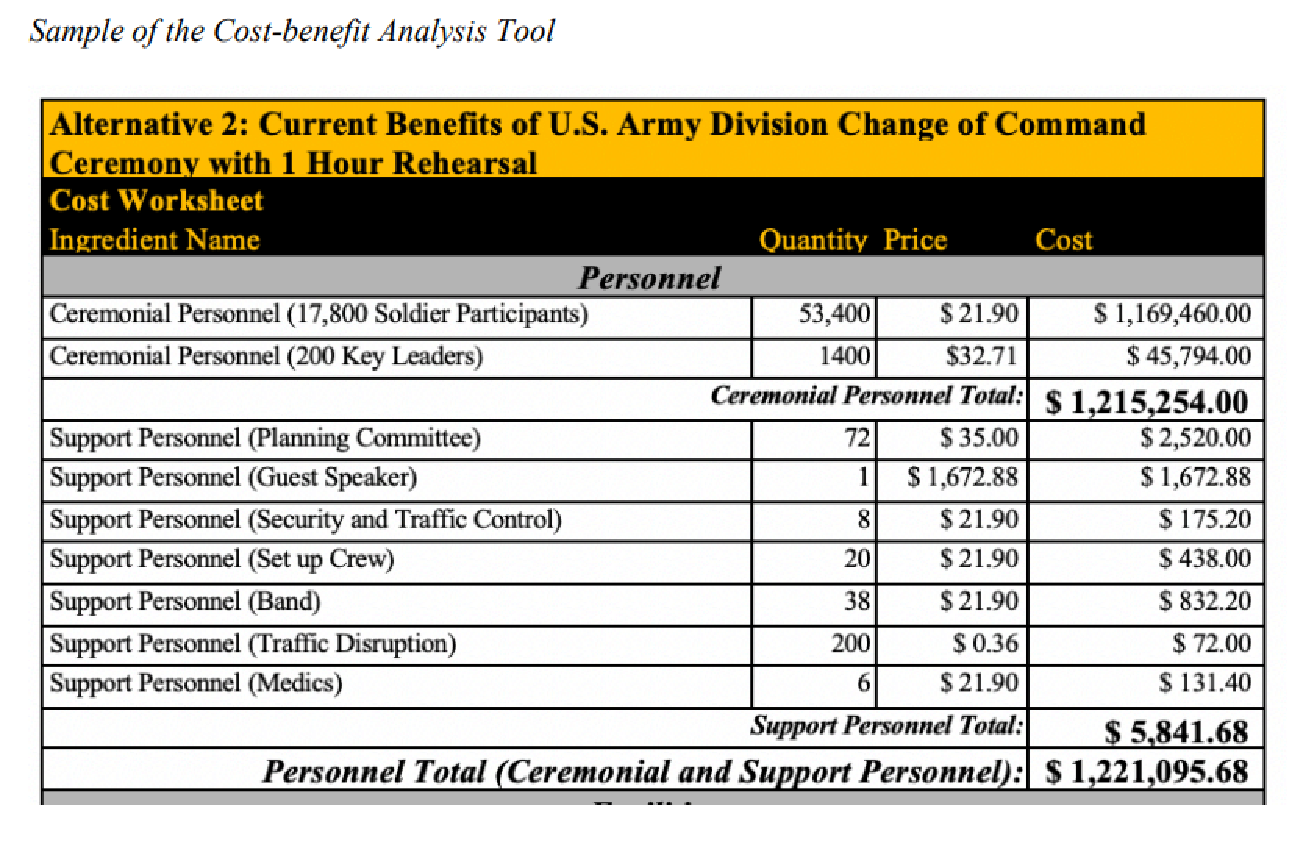
\includegraphics[width=0.4\linewidth,height=0.4\textheight,keepaspectratio]{figures/cost_tool.pdf}
				\caption{Proposed cost tool of \cite{Malin2020}, demonstrating how Army can value Production Loss Costs for different situations.}
				\label{fig:loss_tool}
			\end{figure}

		
		\section{Improving Depot Repair Lead Time Using Lean Six Sigma \cite{Richmond2023}}

			In \cite{Richmond2023}, the author applies Lean Six Sigma to improve the process performance of small government depot repair facility by improving the performance indicators of repair lead time and spares inventory fill rate.

			Richmond discovered that over 80\% of repair lead time was attributed to non-value-added activities, primarily waiting time primarily due to the lack of personnel.
			Through application of Lean Six Sigma tools including DMAIC (Define, Measure, Analyze, Improve, Control), Process Flow Analysis, and 3 x 5 Whys technique, Richmond was able to implement process improvements focused on cross-training, mistake-proofing, and standardizing work.

			After analyzing the current state, the author used a solution selection matrix to determine what solution to implement in a pilot period.
			The implementations included cross training so additional personal could fulfill repair work order tickets, process swimlane improvements, and standardized documentation.
 
			Through the pilot the author showed a decrease in lead times for repairs of 84\% (from 114 days to just 18 days) and inventory fill rate increasing from 54\% to 70\%. 
			This dramatic improvement came primarily from addressing non-value-added waiting times between process steps, which accounted for most of the lead time.

			This case illustrates that lean methodology can be effectively applied to service-oriented, non-aviation Defense maintenance operations, an area with limited prior research. 
			It reinforces the idea that lean principles originally developed for manufacturing can be successfully adapted to maintenance service contexts with appropriate modifications.


		\section{Analyzing Factors That Contribute to Cost Overruns on Department of Defense (DoD) Contractor Programs \cite{FunchesAllen2025}}

			In \cite{FunchesAllen2025}, the author analyzes 524 records of DoD contracts with four machine learning based methods to learn the key factors leading to cost overruns and then make predictions to see which projects were likely to face cost overruns.
			Of the four methods the results revealed that the random forest model achieved the highest accuracy (80\%) in predicting cost overruns. 

			The study identified primary factors contributing to DoD contract cost overruns:
			\begin{itemize}
				\item Inaccurate cost estimation (appearing in 42\% of overrun cases)
				\item Scope modifications (appearing in 11.8\% of overrun cases)
				\item Inadequate risk assessment (appearing in 21.8\% of overrun cases)
				\item Technical issues (appearing in 6.1\% of overrun cases)
				\item Procurement/material issues (appearing in 2.7\% of overrun cases)
			\end{itemize}


			From a lean perspective, these findings align closely with Toyota's focus on waste elimination and continuous improvement. 
			Cost overruns represent a form of financial muda (waste) that stems from imperfections in the planning and execution process.
			The identification of key contributing factors creates opportunities for targeted kaizen (continuous improvement) initiatives within the DoD acquisition system.


	\section{Continuous Learning}

		Building a culture of continuous learning through hansai and kaisen is a cornerstone of the Toyota Way.
		In the digital age, this learning culture can be amplified through digitization of organizational knowledge and data.
		However, a poor approach to such systems can result in the development of waste if information is not easily accessible at the right time, by the right people.

		In the following case studies we see how DoD groups are addressing the existing methods of knowledge base management and data collection to create a lean and effective organization that can do data driven learning.

		\section{Engineering Management Tool for Minimizing Errors and Costs in Diagnosing PTSD in Veterans \cite{Le2023}}

			In \cite{Le2023}, the author developed a Classification Automation Tool (CAT) based on machine learning ensemble methods to improve the accuracy of Post-Traumatic Stress Disorder (PTSD) diagnoses among veterans. 
			The study approached diagnostic errors as a form of waste in Lean engineering terms, with the goal of creating a tool that could assist clinicians in reducing misdiagnoses and associated costs.
			It's important to note that this study focuses on the Veteran Affairs medical process, although the VA is not a department under the DoD it does work closely with the DoD to treat DoD personnel.

			The author demonstrated that using a stacked ensemble machine learning approach resulted in statistically significant reductions in error rates compared to traditional diagnostic methods and other machine learning approaches. 
			In addition the author identified ten predictors connected with PTSD in veterans, including year of birth, purple heart recipient status, gastroesophageal reflux disease (GERD), back pain, joint pain, neck pain, alcohol abuse disorder, bipolar disorder, depression, and mood disorders. 

			The development of the automation tool enables the reduction of defects (misdiagnoses) in a medical process.
			Both false positives and false negatives in PTSD diagnoses represent "muda" (waste) - false positives lead to unnecessary treatments and resource allocation, while false negatives result in delayed care and potentially worse outcomes for veterans.


		\section{Knowledge Management Implementation in U.S. Army Headquarters: A Case Study \cite{VanLaar2023}}

			In \cite{VanLaar2023}, the author conducts a qualitative case study examining the U.S. Army's implementation of knowledge management (KM) as an integrating process within its command and control system. 
			The study focused on how the Army measures knowledge transfer using two assessment tools: the Knowledge Management Maturity Model (KM3) and the Knowledge Management Assessment Tool (KMAT). 

			The analysis by the author revealed that the "people" component of the KM3 model ranked the lowest, indicating that tacit knowledge was not being properly shared within the Army.
			The KMAT was able to identify four primary knowledge transfer barriers: content management issues, personnel turnover impacts, portal use and governance challenges, and the need to anchor KM in institutional governance.

			From a lean perspective, these findings demonstrate how knowledge flow barriers can impede organizational efficiency in ways similar to Toyota's identification of waste (muda) in production systems. 
			At Toyota, tacit knowledge through mentorship is one of the key responsibilities of a manager.


	\section{Stitching the Army's Data Fabric \cite{Patel2021}}

		In \cite{Patel2021}, the authors examine the Army's implementation of data fabric technology to address the challenges of data stovepipes, inefficient data sharing, and the need for rapid decision-making in modern warfare contexts.
		The article describes data fabric as a technology that "stitches" together various information sources and unique data formats, creating a common layer for data discovery, synchronization, and security across multiple platforms and systems.

		The authors identified several critical data management challenges facing the Army: data isolation in warfighting functional systems, compression-induced information loss during data exchange, unnecessarily restrictive classification inheritance, and the inability of AI capabilities to access needed data due to unprocessed and difficult-to-find information.
		These challenges compound the problem of having both too much data and too little usable information for battlefield commanders.

		The Army developed Project Rainmaker to create a tactical data fabric solution.
		Rainmaker prioritizes data synchronization across disadvantaged communications environments and enables AI and machine learning tools to better access and process data for decision support.

		From a lean perspective, the Army's data fabric initiative directly addresses several forms of digital muda (waste).
		Data stovepipes represent waiting waste as users cannot access needed information when required.
		Rather, one should have a pull based data system where data is available on demand by the consuming process or person.

	\section{Out of Sample Examples}

	As the ProQuest dataset included primarily thesis based literature, we wish to diversify the case study sample set. Thus the following section examines an out-of-sample study of lean applications in the DoD.


	% What it is

	% Notable work GigEagle

	% How the DIU displays lean and how specific example displays lean


	\subsection{Defense Innovation Unit and GigEagle}

		Established in 2015, the Defense Innovation Unit (DIU) DIU serves as the DoD's gateway to leading technology companies across the country with offices in Silicon Valley, Boston, Austin, Chicago, and inside the Pentagon.
		Unlike traditional defense acquisition organizations, DIU is the only DoD entity focused exclusively on fielding and scaling commercial technology across the U.S. military at commercial speeds.

		What makes DIU particularly notable from a lean perspective is its streamlined acquisition process. The organization leverages Other Transaction authority (10 USC 4022) to award prototype agreements in as few as 60-90 days \cite{DIU2023workwithus}. 
		Thus the DIU can achieve reduction in cycle time compared to traditional defense acquisition processes that often take years.

		One of DIUs projects is GigEagle. Launched in 2022, GigEagle aims to revolutionize talent management in the DoD by creating a platform that matches DoD organizations with specialized talent from Reserve and National Guard personnel for short-term "gig" projects \cite{GigEagle2022}.

		GigEagle addresses a critical form of waste in the DoD ecosystem: underutilized talent and skills within the Reserve and National Guard components. 
		The platform employs AI/ML technology to automatically match reservist profiles to open requirements posted by DoD organizations. 
		Projects range from four hours to several months in duration, many of which can be staffed remotely. 

		From a lean perspective, GigEagle represents an innovative approach to talent management that emphasizes flexibility, speed, and efficiency.
		By treating talent as a dynamic resource that can flow to where it creates the most value, rather than a static asset bound to traditional organizational structures, DIU has created a system that exemplifies lean principles applied to human capital management in a defense context.


	\section{Conclusion}

		In this report, we examine case studies of how lean/six-sigma principles have been applied across the Department of Defense.
		Our scientometric review has demonstrated that lean and six sigma principles have gained significant traction within the Department of Defense ecosystem, with an increasing trend of publications from 1992 until 2017. 
		Three predominant "lean" themes appeared in the literature: Management and Leadership (54\%), Process Improvement (35.9\%), and Continuous Learning (9.2\%). 
		From those themes we selected a notable examples to present in this report.

		In management and leadership, we observed that traditional command-and-control structures can impede the horizontal communication flows essential to lean organizations.
		However, examples such as the Army's contract management approaches demonstrate that DoD organizations are adapting Toyota-inspired practices, including emphasis on long-term partnerships and feedback loops.

		Process improvement initiatives have shown remarkable results, particularly in depot maintenance operations where lean six sigma implementations achieved an 84\% reduction in lead times. 
		The identification of non-value-added activities and systematic waste elimination mirrors Toyota's kaizen principles. 
		Similarly, the examination of ceremonial costs and contract overruns highlights the DoD's growing recognition of muda in administrative processes.

		The continuous learning theme showcases critical advancements in knowledge management and data accessibility.
		Projects like Rainmaker and the Classification Automation Tool demonstrate how the DoD is addressing information flow barriers—a form of digital muda—to enable more efficient decision-making processes consistent with lean principles.

		Finally, an out-of-sample case study was provided to showcase an example of lean in the DoD which was not included in the literature database. 

		The downward trend in lean six sigma publications since 2017 warrants further investigation. 
		This may reflect either a maturation of lean practices within the DoD, a shift toward alternative improvement methodologies, or potentially reduced emphasis on formal documentation of lean initiatives. 
		Future research should explore this trend and examine whether lean principles have become embedded in organizational culture rather than remaining a distinct improvement initiative.

		In conclusion, while the DoD's hierarchical structure and regulatory environment present unique challenges for lean implementation, this review demonstrates that lean and six sigma methodologies have successfully permeated various aspects of defense operations. 
		The adaptation of Toyota-inspired practices to the defense context suggests that even in highly bureaucratic organizations, lean principles can drive meaningful improvements in efficiency, effectiveness, and organizational learning.

	\newpage

	\bibliographystyle{IEEEtran}
	\nocite{*}
	\bibliography{/project/src/ref}

\end{document}